\documentclass[journal,oneside,a4paper,onecolumn]{IEEEtran}

% Some very useful LaTeX packages include:
% (uncomment the ones you want to load)

% *** CITATION PACKAGES ***
%
\usepackage{cite}
% cite.sty was written by Donald Arseneau
% V1.6 and later of IEEEtran pre-defines the format of the cite.sty package
% \cite{} output to follow that of IEEE. Loading the cite package will
% result in citation numbers being automatically sorted and properly
% "compressed/ranged". e.g., [1], [9], [2], [7], [5], [6] without using
% cite.sty will become [1], [2], [5]--[7], [9] using cite.sty. cite.sty's
% \cite will automatically add leading space, if needed. Use cite.sty's
% noadjust option (cite.sty V3.8 and later) if you want to turn this off.
% cite.sty is already installed on most LaTeX systems. Be sure and use
% version 4.0 (2003-05-27) and later if using hyperref.sty. cite.sty does
% not currently provide for hyperlinked citations.
% The latest version can be obtained at:
% http://www.ctan.org/tex-archive/macros/latex/contrib/cite/
% The documentation is contained in the cite.sty file itself.


% *** GRAPHICS RELATED PACKAGES ***
%
  \usepackage{graphicx}
  \graphicspath{{figs/}}
  \DeclareGraphicsExtensions{.pdf,.png}
  \usepackage{color}

% *** MATH PACKAGES ***
%
\usepackage[cmex10]{amsmath}
% A popular package from the American Mathematical Society that provides
% many useful and powerful commands for dealing with mathematics. If using
% it, be sure to load this package with the cmex10 option to ensure that
% only type 1 fonts will utilized at all point sizes. Without this option,
% it is possible that some math symbols, particularly those within
% footnotes, will be rendered in bitmap form which will result in a
% document that can not be IEEE Xplore compliant!
%
% Also, note that the amsmath package sets \interdisplaylinepenalty to 10000
% thus preventing page breaks from occurring within multiline equations. Use:
%\interdisplaylinepenalty=2500
% after loading amsmath to restore such page breaks as IEEEtran.cls normally
% does. amsmath.sty is already installed on most LaTeX systems. The latest
% version and documentation can be obtained at:
% http://www.ctan.org/tex-archive/macros/latex/required/amslatex/math/

%\usepackage{amssymb}%............................ AMS Symbol fonts



% *** SPECIALIZED LIST PACKAGES ***
%
%\usepackage{algorithmic}
% algorithmic.sty was written by Peter Williams and Rogerio Brito.
% This package provides an algorithmic environment for describing algorithms.
% You can use the algorithmic environment in-text or within a figure
% environment to provide for a floating algorithm. Do NOT use the algorithm
% floating environment provided by algorithm.sty (by the same authors) or
% algorithm2e.sty (by Christophe Fiorio) as IEEE does not use dedicated
% algorithm float types and packages that provide these will not provide
% correct IEEE style captions. The latest version and documentation of
% algorithmic.sty can be obtained at:
% http://www.ctan.org/tex-archive/macros/latex/contrib/algorithms/
% There is also a support site at:
% http://algorithms.berlios.de/index.html
% Also of interest may be the (relatively newer and more customizable)
% algorithmicx.sty package by Szasz Janos:
% http://www.ctan.org/tex-archive/macros/latex/contrib/algorithmicx/

% *** ALIGNMENT PACKAGES ***
%
\usepackage{array}
% Frank Mittelbach's and David Carlisle's array.sty patches and improves
% the standard LaTeX2e array and tabular environments to provide better
% appearance and additional user controls. As the default LaTeX2e table
% generation code is lacking to the point of almost being broken with
% respect to the quality of the end results, all users are strongly
% advised to use an enhanced (at the very least that provided by array.sty)
% set of table tools. array.sty is already installed on most systems. The
% latest version and documentation can be obtained at:
% http://www.ctan.org/tex-archive/macros/latex/required/tools/


\usepackage{mdwmath}
\usepackage{mdwtab}
% Also highly recommended is Mark Wooding's extremely powerful MDW tools,
% especially mdwmath.sty and mdwtab.sty which are used to format equations
% and tables, respectively. The MDWtools set is already installed on most
% LaTeX systems. The lastest version and documentation is available at:
% http://www.ctan.org/tex-archive/macros/latex/contrib/mdwtools/

% IEEEtran contains the IEEEeqnarray family of commands that can be used to
% generate multiline equations as well as matrices, tables, etc., of high
% quality.

% *** SUBFIGURE PACKAGES ***
% subfig.sty, also written by Steven Douglas Cochran, is the modern
% replacement for subfigure.sty. However, subfig.sty requires and
% automatically loads Axel Sommerfeldt's caption.sty which will override
% IEEEtran.cls handling of captions and this will result in nonIEEE style
% figure/table captions. To prevent this problem, be sure and preload
% caption.sty with its "caption=false" package option. This is will preserve
% IEEEtran.cls handing of captions. Version 1.3 (2005/06/28) and later
% (recommended due to many improvements over 1.2) of subfig.sty supports
% the caption=false option directly:
\usepackage[caption=false,font=footnotesize]{subfig}
%
% The latest version and documentation can be obtained at:
% http://www.ctan.org/tex-archive/macros/latex/contrib/subfig/
% The latest version and documentation of caption.sty can be obtained at:
% http://www.ctan.org/tex-archive/macros/latex/contrib/caption/

%Setting captions to centered (Not IEEE journal standard)
\makeatletter
\long\def\@makecaption#1#2{\ifx\@captype\@IEEEtablestring%
\footnotesize\begin{center}{\normalfont\footnotesize #1}\\
{\normalfont\footnotesize\scshape #2}\end{center}%
\@IEEEtablecaptionsepspace
\else
\@IEEEfigurecaptionsepspace
\setbox\@tempboxa\hbox{\normalfont\footnotesize {#1.}~~ #2}%
\ifdim \wd\@tempboxa >\hsize%
\setbox\@tempboxa\hbox{\normalfont\footnotesize {#1.}~~ }%
\parbox[t]{\hsize}{\normalfont\footnotesize \noindent\unhbox\@tempboxa#2}%
\else
\hbox to\hsize{\normalfont\footnotesize\hfil\box\@tempboxa\hfil}\fi\fi}
\makeatother


% *** FLOAT PACKAGES ***
%
\usepackage{fixltx2e}
% fixltx2e, the successor to the earlier fix2col.sty, was written by
% Frank Mittelbach and David Carlisle. This package corrects a few problems
% in the LaTeX2e kernel, the most notable of which is that in current
% LaTeX2e releases, the ordering of single and double column floats is not
% guaranteed to be preserved. Thus, an unpatched LaTeX2e can allow a
% single column figure to be placed prior to an earlier double column
% figure. The latest version and documentation can be found at:
% http://www.ctan.org/tex-archive/macros/latex/base/

% *** PDF, URL AND HYPERLINK PACKAGES ***
%
\usepackage{url}

\usepackage{sistyle}
    \SIstyle{S-Africa}
    \SIunitspace{{\cdot}}
    \SIunitdot{{\cdot}}

% generate nice bookmarks and hyperrefs when exporting to pdf and dvi (screen version):
\usepackage[a4paper,plainpages=false,colorlinks,linktocpage,bookmarks=true,bookmarksopen=false]{hyperref}
% use this for printing only (no color, print version):
%\usepackage[a4paper,plainpages=false,colorlinks=false,linktocpage,bookmarks=true,bookmarksopen=false]{hyperref}

% correct bad hyphenation here
\hyphenation{op-tical net-works semi-conduc-tor}

%List of acronyms used in text
 \usepackage{acronym}%.......................... Acronym package to handle acronyms in text

\acrodef{MMOG}{Massively Multiplayer Online Game}
\acrodef{MMORPG}{Massively Multiplayer Online Role Playing Game}
\acrodef{WoW}{World of Warcraft}
\acrodef{MUD}{Multi-User Dungeon}
\acrodef{PvP}{Player-versus-Player}
\acrodef{P2P}{Peer-to-Peer}
\acrodef{CS}[C/S]{Client/Server}
\acrodef{CMS}[C/MS]{Client/Multi-Server}
\acrodef{NPC}{Non-Player Character}

\begin{document}

%
% paper title
\title{A Scalable Distributed Peer-to-Peer MMOG Architecture}

\author{\IEEEauthorblockN{John S. Gilmore\\}
\IEEEauthorblockA{Department of Electronic Engineering\\
Stellenbosch University\\
Stellenbosch, South Africa\\
Email: jgilmore@ieee.org}}

% make the title area
\maketitle

\begin{abstract}
%\boldmath
The abstract goes here.
\end{abstract}

\hfill May, 2010

\section{Introduction}


\IEEEPARstart{W}{ith} the advent of broadband Internet, \acp{MMOG} have gained significant popularity over the course of the past few years.
Figure \ref{fig_mmog_subscriptions} shows the total number of active MMOG subscriptions over time for the period 1997 to 2008. From here, the accelerating growth of the MMOG market is evident.
%
\begin{figure}[htbp]
 \centering
 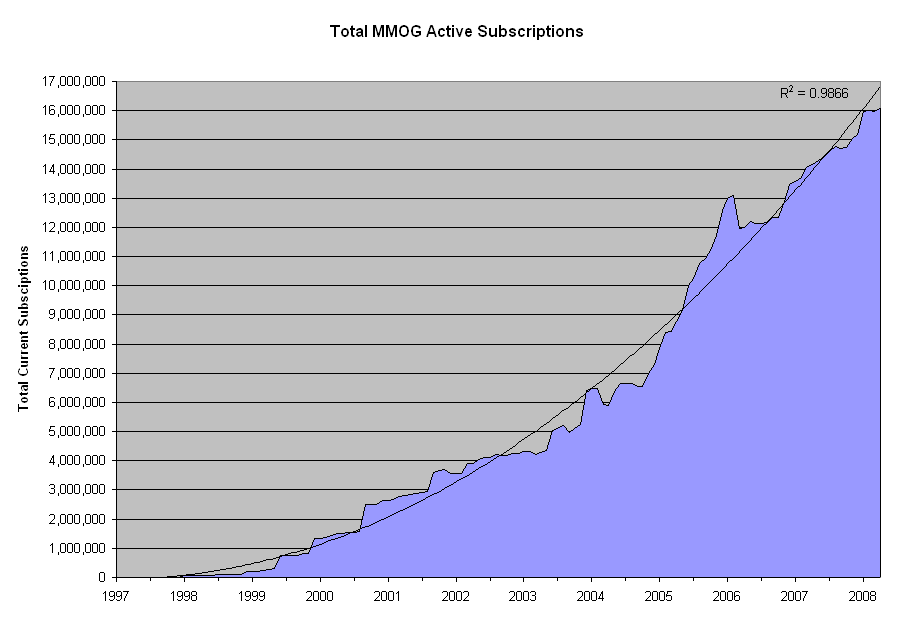
\includegraphics[width=0.5\columnwidth]{MMOG_subscriptions}
 \caption{Total number of active MMOG player subscriptions over time \cite{mmo_growth_chart}.}
 \label{fig_mmog_subscriptions}
\end{figure}

\acp{MMOG} are characterised by expansive worlds, where a large number of players interact online with each other and the virtual environment to achieve certain goals through collaboration and teamwork. Throughout the development of \acp{MMOG}, role play has been tightly coupled to this type of game. This is perhaps due to the exploration and player interaction aspects. Role play allows players to fully immerse themselves in the game world and might, therefore, provide for a more compelling experience. Because of this tight coupling, the terms \ac{MMORPG} and \ac{MMOG} have almost become synonymous. Throughout this work, a distinction will, however, be made between the two.

\acp{MMOG} hold great commercial as well as academic value. From a commercial perspective, the growing number of active subscriptions shown in Figure \ref{fig_mmog_subscriptions} translates to a growing \ac{MMOG} market. Figure \ref{fig_mmog_market} shows the online games market forecast by DFC Intelligence, a company specialising in game market forecasts for various sectors.
%
\begin{figure}[htbp]
 \centering
 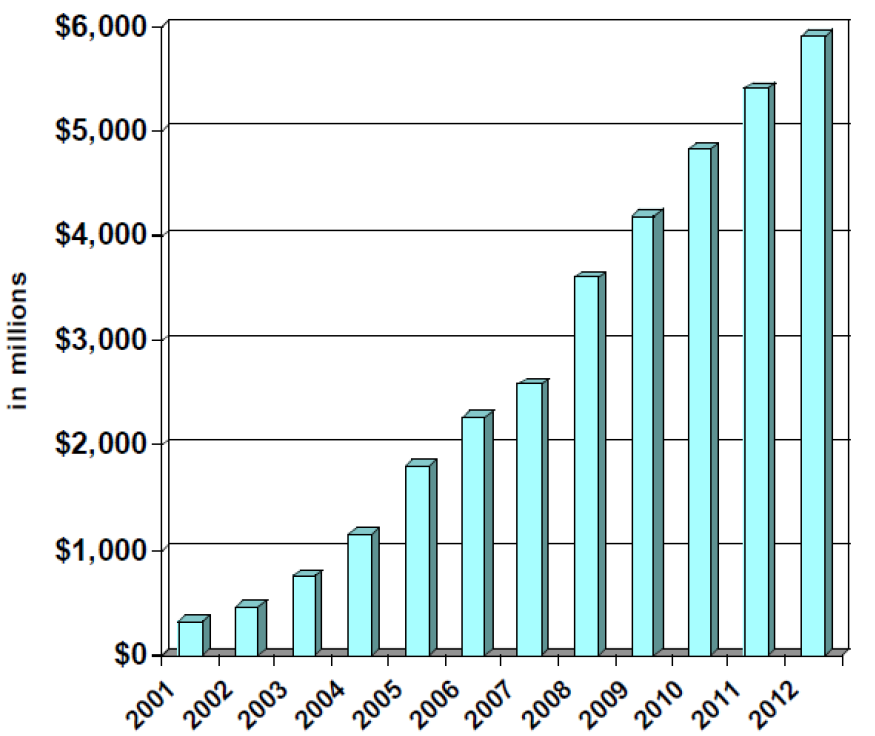
\includegraphics[width=0.5\columnwidth]{DFC_MMOG_market}
 \caption{DFC Intelligence MMOG market forecast '08 \cite{Fan_phd}.}
 \label{fig_mmog_market}
\end{figure}

From an academic perspective, \acp{MMOG} also hold great value. An MMOG is a complex networked application, with clients requiring reliable real-time feedback on actions taken. The design of an MMOG requires in-depth knowledge of server architectures and network design. The design of a server architecture determines how may players the game will be able to host and what the user experience will be in terms of quality of service. The server architecture must be able to handle thousands of requests, store large amounts of data, update the game state and send responses back to all clients in real time.

\section{A brief history of MMORPGs}

\acp{MMOG} have a history stretching from 1978 to the present. A complete history of \acp{MMOG} and the histories of the games and boardgames that they originate from can be found in \cite{mmog_past_present_future} and Chapter 1 of \cite{designing_virtual_worlds}. The first games that could be called \acp{MMOG} were \acp{MUD} (1978) \cite{mud_intro}. \acp{MUD} are entirely text-based, with players exploring areas by receiving descriptions of what they were ``seeing'' and typing commands to move and interact with objects or players. \acp{MUD} contain many of the elements that today are still central to the \ac{MMOG} concept. These elements include exploration, large worlds, multiplayer, social interaction and progression.

After \acp{MUD}, there were many \acp{MMORPG} that acted as building blocks for what is recognised today as being an \ac{MMORPG}. The first graphical \ac{MMORPG} was Neverwinter Nights (1991) \cite{nwn_aol}. Neverwinter Nights was not an Internet based game, it was hosted on what today is the AOL network. Meridian 59 (1994) was the first \ac{MMOG} to have featured a monthly subscription fee, receive wide media coverage and most importantly, the first \ac{MMOG} to feature a 3D engine \cite{meridian59_hist}.

The first \ac{MMORPG} to be commercially successful and largely credited with popularising the genre was Ultima Online (1997). Ultima Online used existing intellectual property from the Ultima universe as well as an aggressive marketing campaign by game publisher EA, to quickly gain 100,000 subscribers. NCsoft's Lineage (1998) looked similar to Ultima Online, but was more \ac{PvP} oriented and with an added castle siege mechanism, became very popular in South Korea. Lineage had more than three million subscribers at one point, most of them from South Korea \cite{mmog_subscriptions}. Everquest (1999) is credited for bringing \acp{MMORPG} into mainstream Western Culture. It featured a large persistent 3D environment that was capable of hosting up to 15000 players per server \cite{everquest2_capacity}.

\acp{MMORPG} in the first millennium are considered to be of the first generation. These games provided blueprints for all \acp{MMORPG}
to follow in the second generation. While there are many more games in the second generation, these games are characterised by little innovation
in the genre and focus more on improving graphics and ease-of-use \cite{mmog_past_present_future}. Notable games in this generation are: Final Fantasy XI (2000) (console based), Dark Age of Camelot (2001) (realm vs. realm combat) and Anarchy Online (2001) (instancing).

Eve Online (2003), developed by CCP Games in Iceland, brought many new innovations to the \ac{MMORPG}. It was the first successful MMORPG to feature a science fiction theme. It was the first MMOG to have a single distributed server architecture. This meant that no sharding was required. Sharding is a method by which the game world is duplicated onto multiple servers to distribute load. Players cannot communicate between shards as these worlds are complectly isolated from each other. By employing a distributed server architecture, where different regions of the virtual world was hosted on different servers, players could have a seamless and more immersive experience. This was accomplished by hosting different star systems on different servers. Players have to use a warp gate to travel between star systems. This mechanic is used to mask the time it takes to move the player from one server to another. In 2006, CCP Games launched the largest supercomputer in the gaming industry to upgrade their existing infrastructure and enable Eve to support more than 50,000 concurrent users \cite{eve_launces_supcom}. This number that was surpassed in 2009 with 54,181 concurrent users in game \cite{eve_pcu}.

Another innovation of Eve was the in-game economy. CCP games appointed Dr. Eyj\'{o}lfur Gu\~{o}mundsson as chief economist of Eve online in 2006 \cite{eve_economist}. His duties were to monitor and predict market trends in the game world and produce detailed quarterly economic reports \cite{eve_econ_rep}.  The economy is based on a open market system ruled by supply and demand. No other game has implemented an in-game economy in such a rigourous fashion.

Blizzards's \ac{WoW} (2004) is the most successful MMORPG to date. After six years it still has by far the most subscribers of any MMOG, totaling 11,5 million, each paying \$15 per month subscription \cite{wow_subscibers}. In 2008 it was estimated that WoW holds more than 60\% of the MMORPG subscription market \cite{mmog_sub_market}. From the first generation of games, a steady growth has been seen in the MMOG space, but before the run away success of WoW, no one had estimated that the gaming market could be this large \cite{mmog_growth_analysis}. It should be noted, however, that the growth seen in the \ac{MMOG} market, is mostly due to growth in the Asian markets and that the size of these markets are much larger than the size of the Western markets.

The success of \ac{WoW} has largely been attributed to the overall quality and finish of the game \cite{wow_csf}. It is interesting to note that WoW is not attributed with many innovations. Most games that came before it implemented most of the features in WoW. What WoW did do, is combine all previous innovations into a package that was accessible to a large number of people.  Players also don't just play WoW to experience the game content, they also play the game to meet up with friends and socialise. Guilds are also an integral part of WoW. Guilds are collections of players that choose to play together to achieve some common goal.

\section{Overview of MMOG network architectures}

The previous section presented a brief history of the \ac{MMOG} and more specifically, the \ac{MMORPG} genre. This section explores the network architectures that are generally employed by this genre of games. The network architecture of a system specifies how the different entities in the network communicate, where authority lies and whether a centralised or distributed approach is followed. Currently, all MMOGs being operated run on a \ac{CS} architecture or a distributed \ac{CS} architecture, also called a \ac{CMS} architecture. The simplest form of network architectures used in MMOGs is the pure \ac{CS} model.

Figure \ref{fig_cs_arch} shows the \ac{CS} model. The server is the entity on which the MMOG is hosted and is controlled by the game producer. Clients are computers operated by players, that connect to the server to play the game. The server is responsible for updating the game state, according to client actions, to store the new game state and to distribute game state updates to all clients. An in-depth exploration of consistency models, of which this theory forms part, will be presented in Section \ref{consistency_models}. Clients never communicate with other clients. They send their actions to the server and receive the updated states of other players from the server.

The \ac{CS} architecture has two main advantages that made it the architecture of choice for all MMOG developers. Because of the centralised approach of the architecture, both administration and security are greatly simplified. Administration is simplified, because the game producer has full control over the server, server data and code. It controls physical access as well as which clients are allowed to connect the the system. Efficient logging is also supported, because the server is able to not only log all server actions, but also all client actions, since these also pass to the server.

Security is a significant issue in MMOGs, since some players sell in-game currency for real-world currency \cite{}. This makes the MMOG a platform that is capable of producing income, which increases the incentive of players to be able to gain an unfair advantage over other players. The more popular an MMOG, the greater the security threat. Because the producer has full control over the server code and is never required to furnish the client with the server code, it makes it difficult for a potential attacker to use knowledge of the server in an attack. Because clients are never allowed to communicate, all malicious users can be filtered out of the network by the server when detected and even banned from the network. Producers are able to ban players, because these games usually require a game account, which is linked to a copy of the game as well as some payment method. This introduces a large cost to player whose accounts are banned.

The \ac{CS} architecture however does have some disadvantages. These are weak robustness, weak scalability, high cost to the provider, high latency, high amount of required server bandwidth and weak handling of transient loads. The robustness of the system is weak because it is a single point of failure. If the server fails or goes down for maintenance, the game is off-line and players are unable to play. 

This system is also not scalable, since a single server cannot easily be extended with more resources. Even if an off-line approach is used, where hardware is upgraded after the system is taken down for maintenance, the hardware required to support a game hosting more than 300 players, become prohibitively expensive \cite{}. The problem leads to the weak handling of transient peak loads. Players prefer playing during certain times and usually after a game patch has been released, the players load increases for a short period of time. The server hardware should be able to support peak system loads, which means that sufficient resources shoud always be provisioned to support these peak load. This is not an economically viable solution, because resources to handle peak loads are not used most of the time. This translates to producers paying for the provisioning of resources, without having active players that pay for these resources.

This disadvantage also leads to the next one, namely high cost for the provider, which translates to high costs for clients or reduced profit. The cost come from the hardware that is required to host the system as well as maintenance and running costs. Running costs include bandwidth provisioning and IT personnel and maintenance costs include replacement of malfunctioning or outdated hardware. It has been estimated that maintenance and running costs consume approximately 80\% of game revenue during the lifetime of the game \cite{}.

Because no clients are allowed to communicate with other clients, every change that is made to the game world by a client, first had to be communicated to the server, which in turns relays this message to all clients after applying game logic and artificial intelligence (AI) algorithms. This two hop path, with the additional time for computation added by the server as well as possible buffering at the server when many clients communicate, significantly increases the latency of the system compared to a system where direct communication is used.


In an effort to address some of these issues, the distributed \ac{CS}, also called \ac{CMS}, was introduced. In a distributed \ac{CS} model, the server functions are distributed amongst multiple machines in an effort to distribute the server load. For MMOGs, there are various methods employed to achieve this. One of the first methods used is called sharding, where copies of the game world run on different servers and clients connect to one of these shards \cite{}. Clients are not able to interact or communicate with players on other shards, which reduces game immersion. This method does, however, allow for a more scalable system as maximum load is fixed. Players are not able to enter a shard if that shard has reached it capacity. This has in the past caused unhappiness amongst players, since popular shards could be difficult to log in to. Players are also reluctant to move to a new shard, because a lot of time is invested in their characters in their ``home'' shard. For all practical purposes, this approach is still merely a \ac{CS} approach, with players forced into specific \ac{CS} environment.

%Redundant
There are three popular true distributed models used in MMOGs today. These are redundancy based, region based and object based \cite{}. The first one is very similar to sharding, with the difference that all server share the same duplicated game state. Each server contains the global game state and clients connect randomly or through some sort of load distribution algorithm to a server. Each server handles all actions from clients and updates its own database. The servers in turn send updates to each other over a high quality link, such as fibre, to maintain database consistency at high speeds. The problem with this system is that the world is never truly consistent and that there are no optimally chosen inconsistency obfuscation boundaries. In other words, two players standing next to each other in the virtual world, might be on different servers and, therefore, experience two different worlds. Game inconsistency is not necessarily an issue, but then it should be based on a distance based approach where the consistency degrades gracefully the greater the distance between players in the virtual world. This system is also not truly scalable because of the large hardware costs involved in the system as well as network hardware required to achieve sufficient performance for large numbers of players.

%Region based
Another method that has also been employed is to divide the virtual world up into regions and host the different regions on different servers \cite{}. Busy regions are hosted on their own servers, while multiple quiet regions are hosted on a single server. The issue of this static region approach is that it also does not scale well when one region is suddenly populated with players. This type of behaviour happens quite regularly and is known as flocking \cite{}. When players find something of interest in a region, many players will flock to that region. In-game events and festivals are also becoming popular and these events also cause flocking to the region where the event is held. The solution to these effects have been over provisioning of resources to handle peak loads, which suffers from the disadvantages discussed above. Also, if the load changes, the server has to be brought off-line in order to rebalance the regions. Dynamic regions are being investigated, where regions can be dynamically shifted from one server to another, in order to balance load \cite{}. This approach unfortunately causes a lot of overhead and adds significant complexity with regards to the migration of the data and the handling of player actions while the data are in transit \cite{}.

%Object based
The third method used is to distribute all in-game objects amongst the servers. For an MMOG, most of these objects are expected to be players objects. The advantage of this method is that the system load is fixed for a certain player population and that the load is equally distributed amongst all server. This allows for more accurate prediction and provisioning  of required resources, but still does not handle transient loads well. Another issue is inter-server communications for this architecture. The inter-server communications are random and also much more than the inter-server communications for a region based system. The reason for this is that the amount of player interaction increases with a decrease in the distance between the players. Players playing together move together, chat and interact with \acp{NPC} together. For a region based model, all player interaction near to each other remain in the server.

In general, the issues addressed and improved by the \ac{CMS} architecture are robustness, scalability, and peak load handling. The system is more robust, because the failure of one server will not necessarily lead to the failure of the whole system for certain system designs. The system is more scalable, because many less powerful servers may be used, which allows for the hosting of more players than what is currently possible with single server hardware. It also handles transient loads better, because, for cases where loads can be predicted, resources can by shifter between servers to improve the user experience.

The disadvantages of this system is that the administration complexity is greatly increased. Such systems, although capable of handling many more users than a single server, is also much more expensive. These disadvantages are however not technical problems and so it is assumed for current games, that these systems are what is required if a game is to be hosted for a large number of players.

\section{Peer-to-Peer MMOG architectures}
\subsection{Overview}

Recently, an alternative architecture has gained popularity, making use of a peer-to-peer architecture to host the MMOG \cite{}. This has opened up a new research field that is attempting to make the peer-to-peer model a viable alternative to the classic \ac{CS} and \ac{CMS} architectures. This architecture does, however, still have a few major issues that need to be solved before MMOGs can be developed that use it. If these issues, which are later discussed, can be solved, a \ac{P2P} architecture holds some powerful advantages over a \ac{CS} system.

The core idea of the \ac{P2P} model is that each peer contributes enough resources to the network to be able to host itself. This also means that all functions of the server in the classic \ac{CS} model are distributed amongst all peers. There are many areas where the \ac{P2P} model can improve on the classic \ac{CS} model. These areas are robustness, scalability, provider cost, latency, server bandwidth and handling of peak transient load.

The system is very robust, because there is no server that can fail, only individual peers. Individual peers failing will not affect any other peers other than the peer that failed. This behaviour makes game down-time extremely unlikely.

Also, because every peer is expected to add sufficient resources to the system to host itself, this makes the system very scalable with no extra costs being incurred from a provider viewpoint for any peer that joins the network. This will also allow for efficient handling of transient loads. If many players suddenly enter the game, no resourcing provisioning issues will arise, as peer bring the resources they need with them into the system. It should also be noted that it is not at all unreasonable that a peer will have sufficient resources to host itself. Peer computers are very powerful systems these days, with multi-core CPUs, multiple gigahertz of clock speeds, multiple gigabytes of memory and secondary storage space in the terabyte range. The graphics cards in gaming machines have also become immensely powerful. With such a system in mind as the average gaming system, it is not unreasonable to assume that sufficient resources will be available.

\ac{P2P} architectures also create a lot of opportunity for independent developers, because a large initial investment is now no longer required to purchase the expensive server hardware. Not just are hardware costs greatly reduced, but running costs are also greatly reduced. The bandwidth required by the game server is now shared amongst users. Which means that no bandwidth costs will be incurred by the provider. Also, the amount of required bandwidth per user is usually not high, which means that users will not be expected to use a much greater amount of bandwidth.

Latency is also improved, because it is now possible to directly communicate between peers and not neccesary to go through a server for communications. There is also no single server that has to process peer actions. Peer actions need only be processed by other peers who find the specific peer actions of interest. The distribution of the load as well as direct communication will reduce latency.

\begin{table}[htbp]
\centering
\begin{tabular}{|r|c|c|c|}
\hline
Property & Client/Server & Client/Multi-Server & Peer-to-Peer\\
\hline
Administration & Simple & Challenging & Complex\\
Security & High & High & Low\\
Robustness & Low & Medium & High\\
Scalability & Low & Medium & High\\
Provider cost & High & Very high & Low\\
Latency & High & High & Low\\
Server bandwidth & High & High & None\\
Peer bandwidth & Low & Low & Medium\\
Peak transient load handling & Bad & Medium & Good\\
\hline
\end{tabular}
\caption{Differences between Client/Server, Client/Multi-Server and Peer-to-Peer architectures}
\label{tab_archs}
\end{table}

Table \ref{tab_archs} summarises the differences between the three architectures as discussed thus far. What remains to be said is why administration and security were marked as complex and low respectively. From an administrative perspective, it is more complex to administer a decentralised system than a centralised one \cite{}. The reason is that the game producer has full control over the server in the \ac{CS} architecture. The administration tools only have to control the centralised server or server cluster. For a peer-to-peer system, the server is the collection of all peers. The game producer does not have direct access to peers and so controlling these nodes become significantly more complex.

The server or cluster is housed in a secured location, where access can be controlled. As stated earlier, the server code is also protected and not accessible to potentially malicious players. These factors simplify the security of the \ac{CS} model by allowing the developers to place all intelligence in the server and move all sensitive computations to the server. Clients do not house game logic and the client state is also not authoritative.

If this model is contrasted with a P2P model, the P2P model has some significant security challenges \cite{}. The challenges reside in the fact that peers are not under the control of the game producer. Since all server data are distributed amongst peers, all peers have access to sections of the server data. Peers also have access to the distributed server code. One advantage that can be exploited is that no peer contains all server data and no one peer has more authority than another. This allows for schemes such as quorum algorithms to be used to increase the security level. This and other techniques are discussed in Section \ref{}.

\subsection{Key challenges}



\section{Proposed architecture}

\section{Consistency models}
\label{consistency_models}

\section{Proposed state persistency model}

\section{Related work}

\section{Contributions}

\section{Conclusion}
The conclusion goes here.

\bibliographystyle{IEEEtran}
\bibliography{P2P_MMOG}

% that's all folks
\end{document}


